\section{Materiales y Métodos}
% \section{Leyes de conservación hiperbólicas escalares}

\begin{frame}
	\frametitle{\secname}
	Consideramos el Beam-Warming definido por
	\begin{equation*}
		u_{i}^{n+1}=
		u_{i}^{n}+
		\sigma(2-\sigma)
		\left(u_{i-1}^n-u_i^n\right)+
		\frac{\sigma}{2}(\sigma-1)
		\left(u_{i-2}^{n}-u_{i}^{n}\right)
	\end{equation*}

	\begin{enumerate}
		\item

		      Reescriba el esquema como una corrección al esquema FOU, con los
		      términos adicionales bajo la forma de diferencias entre puntos adyacentes
		      \begin{equation*}
			      u_{i}^{n+1}=
			      \underbrace{
				      u_{i}^{n}-
				      \sigma\left(u_i^n-u_{i-1}^n\right)}_{\text{Esquema Monótono}}-
			      \underbrace{
				      \frac{\sigma}{2}
				      \left(1-\sigma\right)
				      \left(u_{i}^{n}-u_{i-1}^{n}\right)+
				      \frac{\sigma}{2}
				      \left(1-\sigma\right)
				      \left(u_{i-1}^{n}-u_{i-2}^{n}\right)}_{\text {Términos no monótonos}}
		      \end{equation*}

		\item

		      Multiplique los dos términos no monótonos por las funciones
		      $\Psi\left(r_{i}\right)$ y $\Psi\left(r_{i-1}\right)$,
		      lo que resulta en
		      \begin{align*}
			      u_{i}^{n+1} & =
			      u_{i}^{n}-
			      \sigma\left(u_i^n-u_{i-1}^n\right)-
			      \frac{\sigma}{2}
			      \left(1-\sigma\right)
			      \Psi\left(r_{i}\right)
			      \left(u_{i}^{n}-u_{i-1}^{n}\right)+
			      \frac{\sigma}{2}
			      \left(1-\sigma\right)
			      \Psi\left(r_{i-1}\right)
			      \left(u_{i-1}^{n}-u_{i-2}^{n}\right).
		      \end{align*}

		\item
		      Este esquema limitado será monótono si el término entre
		      corchetes es positivo, lo que lleva a la condición
		      \begin{equation*}
			      \frac{\Psi\left(r_{i-1}\right)}{r_{i-1}}-
			      \Psi\left(r_{i}\right)\leq
			      \frac{2}{1-\sigma}.
		      \end{equation*}
		      Esta relación es satisfecha con la condición
		      \begin{equation*}
			      0\leq\Psi\left(r\right)\leq
			      \min\left\{\frac{2r}{\sigma},\frac{2}{1-\sigma}\right\}.
		      \end{equation*}
	\end{enumerate}
\end{frame}

\begin{frame}
	\frametitle{\secname :Diagrama TVD de Sweby}

	\begin{figure}[ht!]
		\centering
		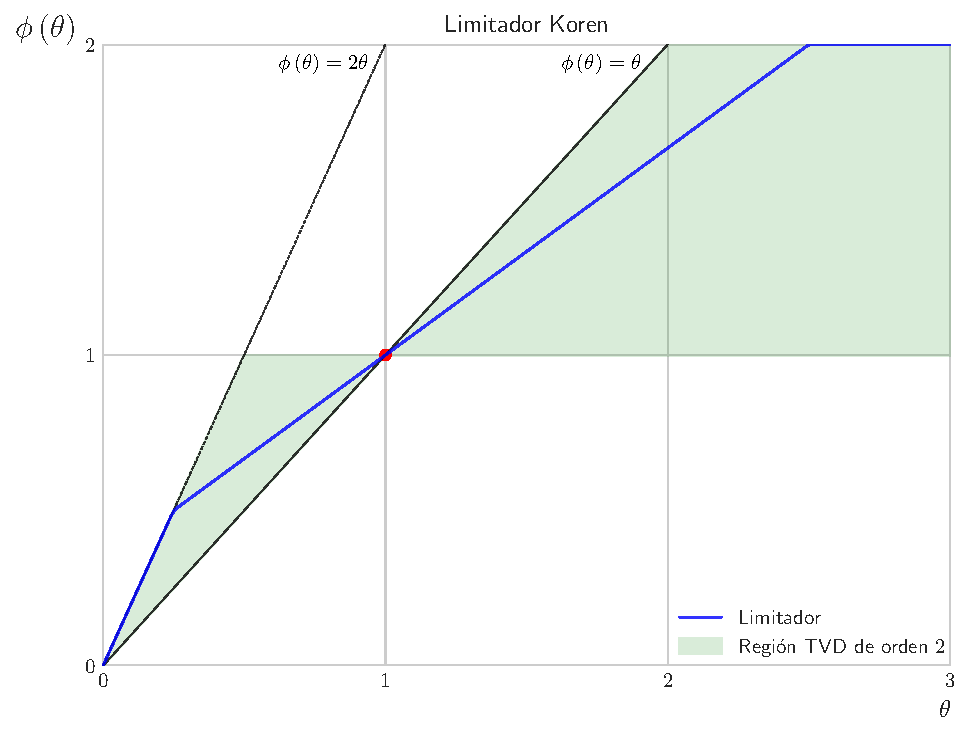
\includegraphics[width=.38\paperwidth]{limiterkoren}
		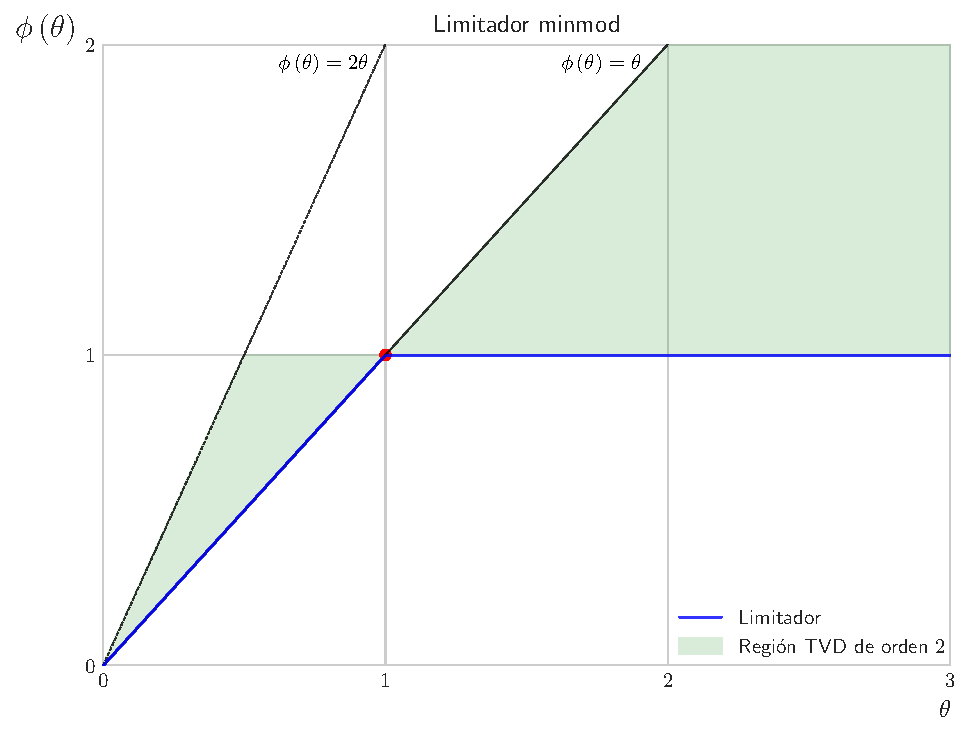
\includegraphics[width=.38\paperwidth]{limiterminmod}
		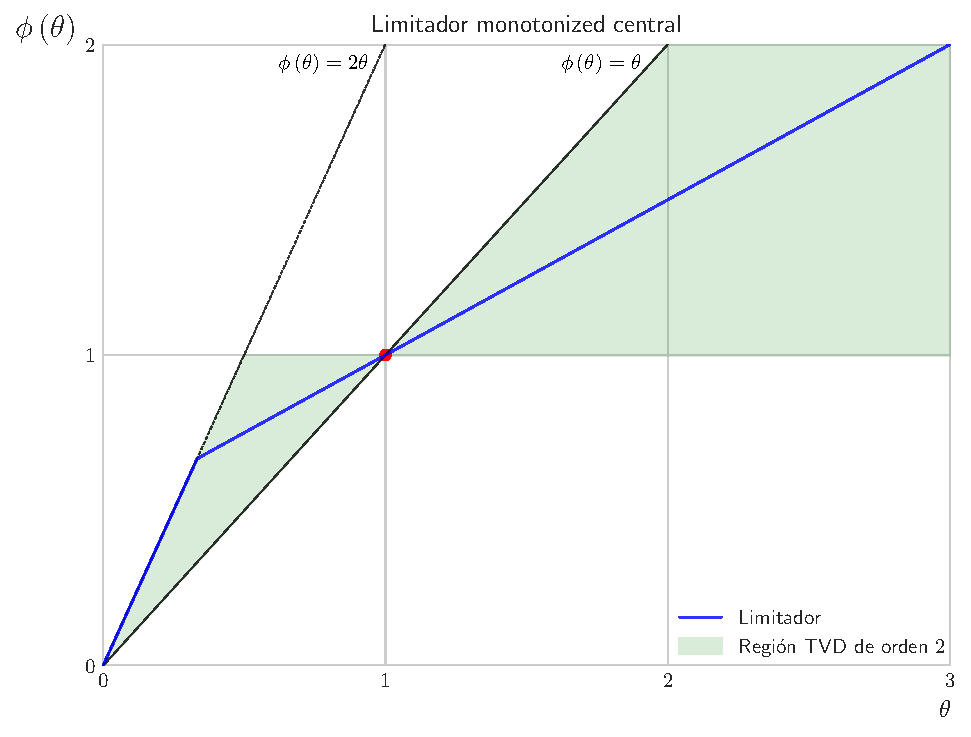
\includegraphics[width=.38\paperwidth]{limitermonotonizedcentral}
		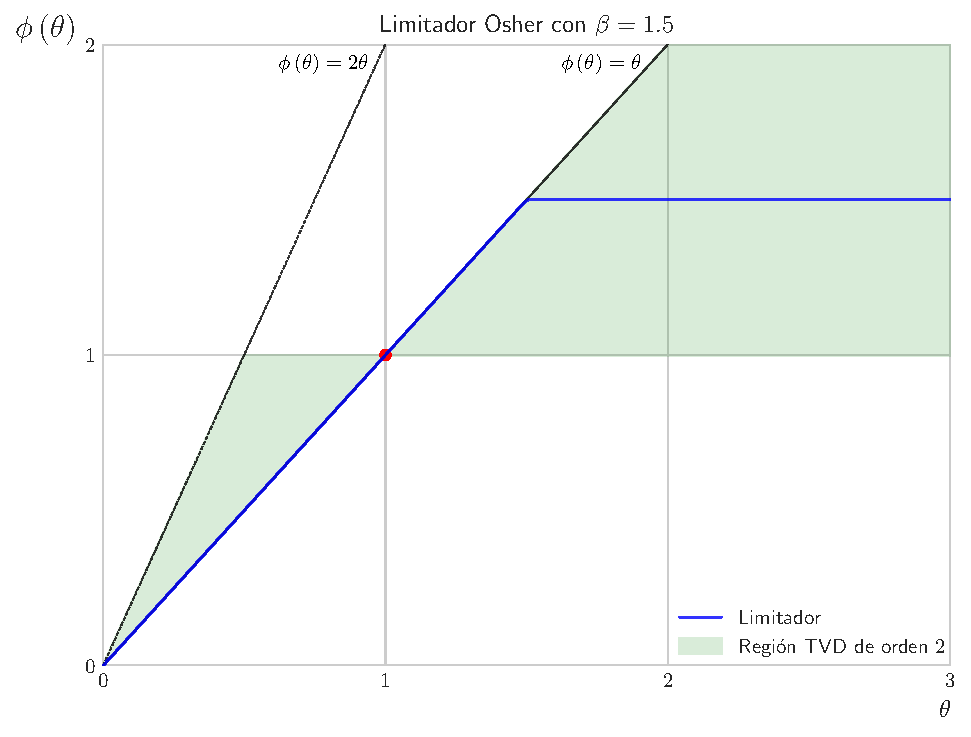
\includegraphics[width=.38\paperwidth]{limiterosher}
	\end{figure}
\end{frame}


\begin{frame}
	\frametitle{\secname :Diagrama TVD de Sweby}

	\begin{figure}[ht!]
		\centering
		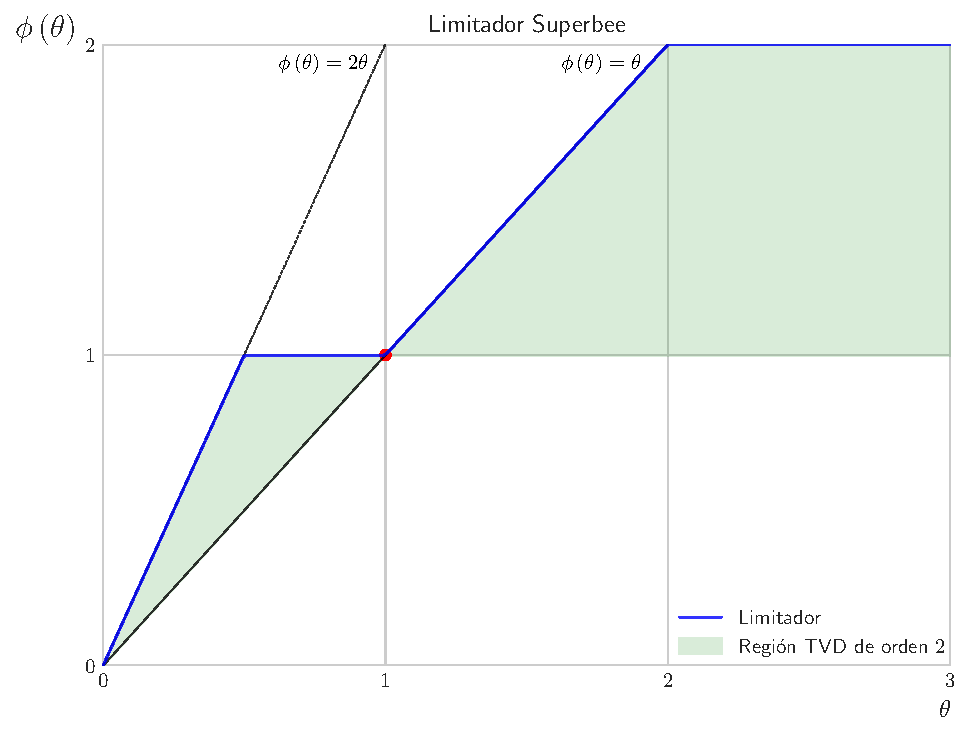
\includegraphics[width=.38\paperwidth]{limitersuperbee}
		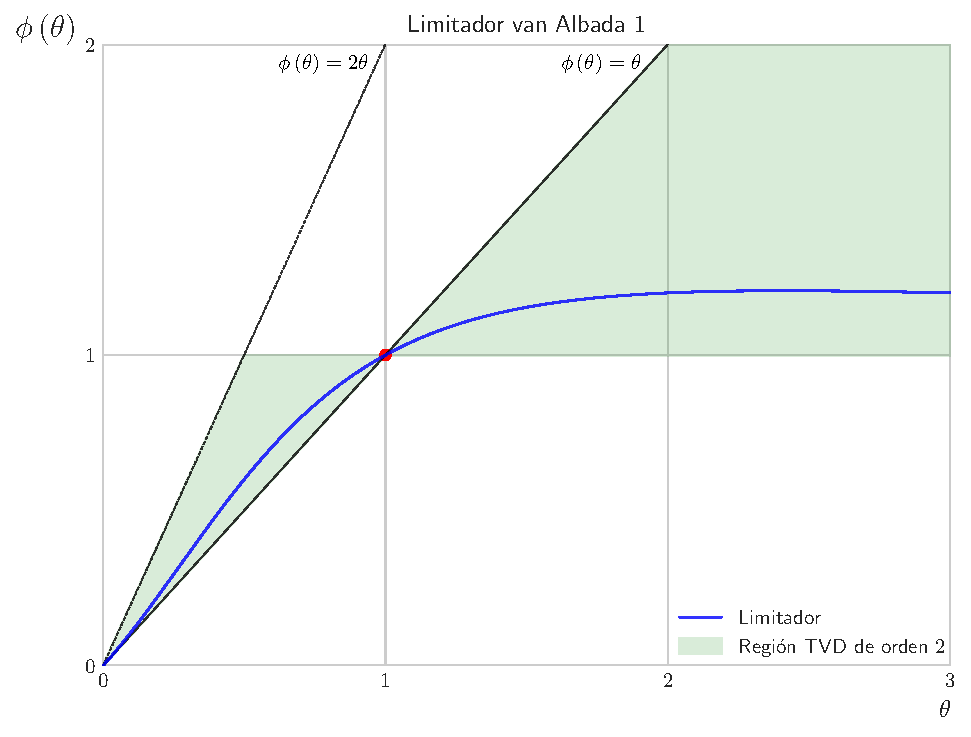
\includegraphics[width=.38\paperwidth]{limitervanalbada1}
		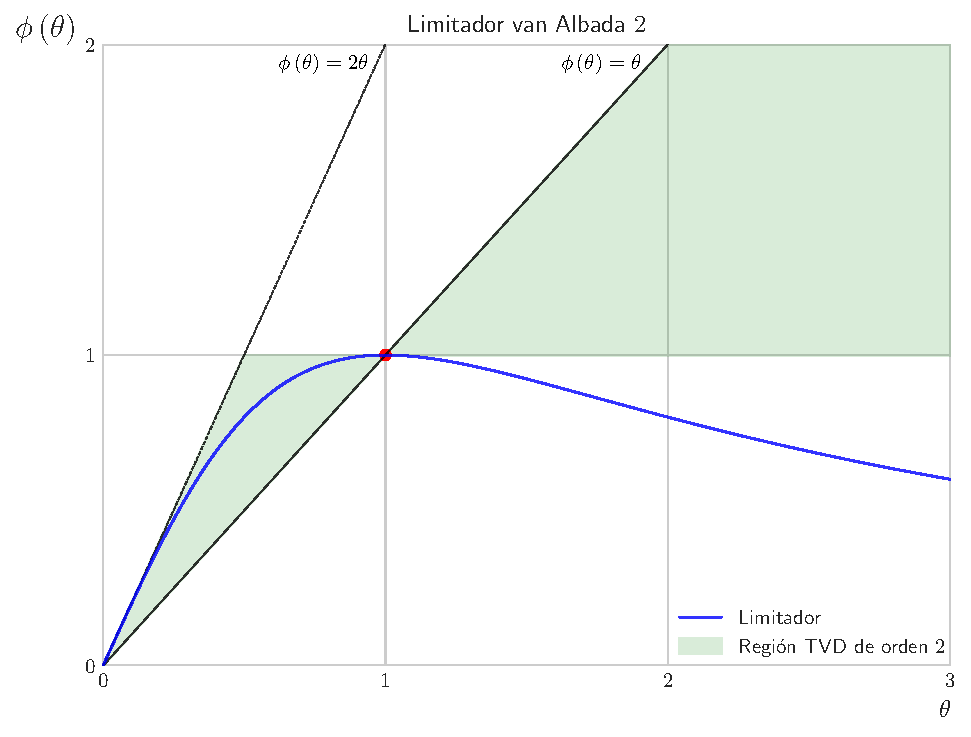
\includegraphics[width=.38\paperwidth]{limitervanalbada2}
		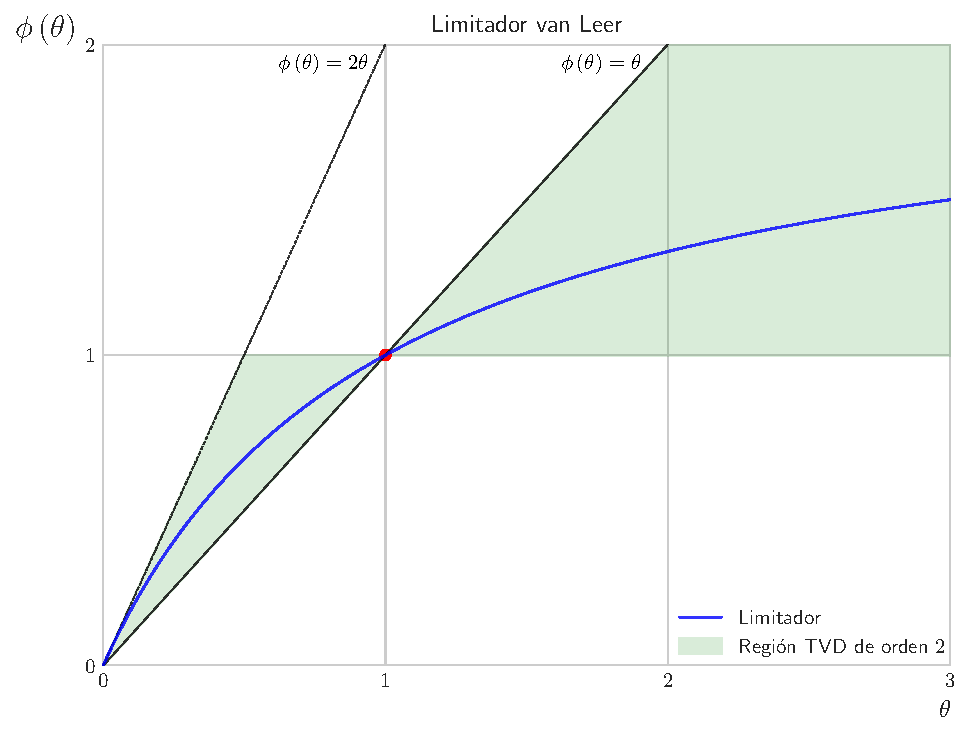
\includegraphics[width=.38\paperwidth]{limitervanleer}
	\end{figure}
\end{frame}
